\clearpage

\AddToShipoutPictureBG{
    \begin{tikzpicture}[remember picture, overlay]
        \node[opacity=0.08] at (current page.center) {
            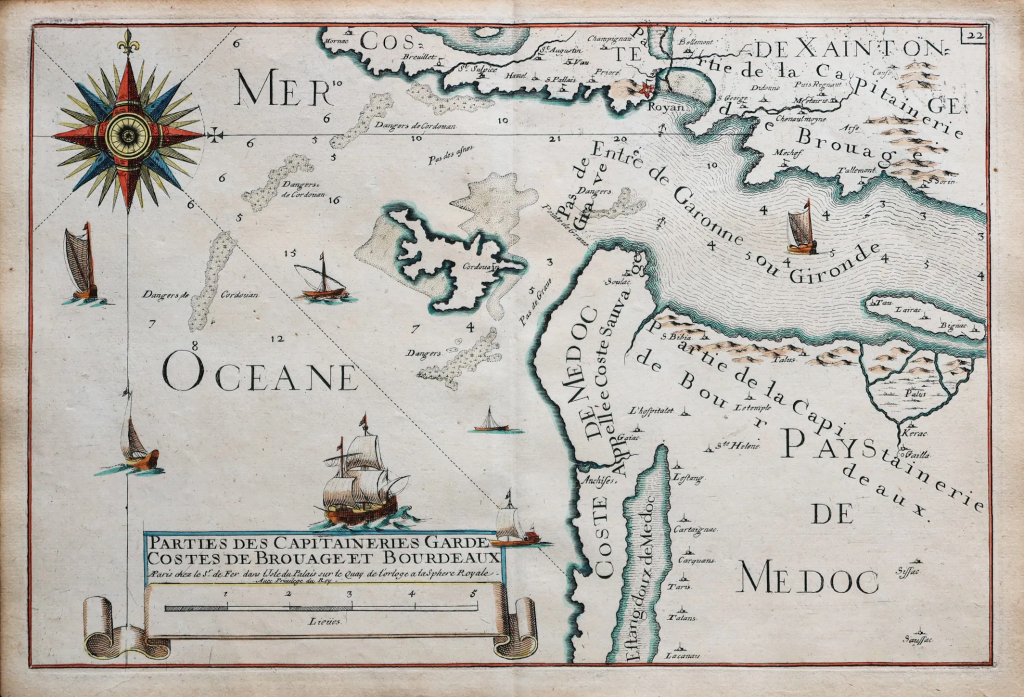
\includegraphics[width=\paperwidth,height=\paperheight]{image/carte-maritine}
        };
    \end{tikzpicture}
}

\chapter{Contrat individuel d'apprentissage}
\label{chap:contrat_apprentissage}

Le contrat individuel d'apprentissage, établi au commencement de l'année académique et validé par le professeur référent, constitue la carte de navigation de la démarche présentée dans ce portfolio. Sa version intégrale est jointe en \textbf{annexe A}. Le présent chapitre n'en reproduit pas le détail ; il en expose les lignes directrices, les choix déterminants et leur cohérence avec les compétences retenues.

\section{Cap pédagogique et compétences retenues}

Le cap pédagogique fixé au début du parcours repose sur une finalité claire : dépasser le registre strictement technique pour évoluer vers une professionnalité transdisciplinaire, capable d'articuler conception, collaboration, cadrage stratégique et mise en œuvre.

Dans cette perspective, trois compétences ont été arrimées comme points d'ancrage. Leur justification détaillée est présentée dans l'introduction, à la section \textit{Trois compétences, trois chantiers} (voir section~\ref{sec:trois-competences-justification}) :

\begin{itemize}
    \item \textbf{A2} (gestion des divergences et facilitation de la convergence), pour renforcer la délégation, la coopération et la prise de décision collective.
    \item \textbf{B4} (méthodes agiles au service du prototypage itératif), pour structurer l'apprentissage par la pratique et piloter les itérations avec méthode.
    \item \textbf{C2} (synthèse et définition des problématiques prioritaires), pour affiner la capacité à poser un diagnostic pertinent avant d'orienter une réponse.
\end{itemize}

Ces trois compétences forment la quille du parcours développemental : elles soutiennent la progression attendue et assurent une cohérence entre intentions initiales, activités de formation et critères d'autoévaluation.

\section{Logique d'alignement entre objectifs et choix de cours}

Mes objectifs pédagogiques personnels se concentrent sur trois axes :

\begin{itemize}
    \item développer une conception centrée utilisateur et une meilleure lisibilité des solutions proposées ;
    \item améliorer la capacité à défendre un projet, à argumenter sa valeur et à l'inscrire dans une logique de marché ;
    \item progresser dans la collaboration, la délégation et la conduite collective des projets.
\end{itemize}

Le choix des cours à option répond directement à cet agencement d'objectifs et fait écho aux compétences justifiées dans l'introduction :

\begin{description}
    \item[\textbf{Méthode de recherche 1, 2 et 3}] repère analytique pour investiguer le terrain, clarifier les besoins et nourrir prioritairement la compétence \textbf{C2}.
    \item[\textbf{Médiation}] appui central pour traiter les divergences, parvenir à des accords opératoires et renforcer la compétence \textbf{A2}.
    \item[\textbf{Gestion de projet 1, 2 et 3}] cadre méthodologique pour conduire des cycles itératifs et consolider la compétence \textbf{B4}.
    \item[\textbf{Gestion financière 1 et 2}] appui de pilotage pour relier faisabilité économique, arbitrages de projet et argumentation auprès des décideurs, en soutien transversal des trois compétences.
    \item[\textbf{Technique de vente et négociation}] deux compétences que mon profil d'ingénieur n'a jamais cultivées, mais indispensables pour défendre la valeur d'une solution, convaincre des décideurs et négocier dans des contextes professionnels. Ces cours comblent directement la brèche entre l'expertise technique et la capacité à la valoriser.
    \item[\textbf{Start-up et industrialisation}] pont entre l'intuition entrepreneuriale acquise sur le terrain et un cadre structuré pour penser le passage d'une idée à un produit viable ; ancrage dans la réalité des deux univers que j'ai traversés.
    \item[\textbf{Droit des sociétés et protection intellectuelle}] deux angles d'un même angle mort : ne pas savoir cadrer juridiquement une initiative ou protéger ce qu'on crée est un frein réel à toute ambition de dépasser le rôle d'exécutant. Ces cours apportent les fondations manquantes.
    \item[\textbf{Communication au sein d'une institution}] compétence éprouvée sous sa face la plus difficile lors de restructurations subies ; comprendre ses mécanismes pour ne plus en être le simple objet mais un acteur capable d'y naviguer.
    \item[\textbf{Méthode de veille}] domaine qui me passionne depuis que j'ai mis en place des outils d'aide à la décision stratégique ; l'approfondir nourrit directement la compétence \textbf{C2} et la capacité à cadrer les bons problèmes.
    \item[\textbf{Prototypage et produit physique}] lacune assumée d'un ingénieur logiciel : penser par le faire, avec des contraintes matérielles, change profondément la manière d'innover et d'itérer.
    \item[\textbf{Vidéo et art oratoire}] deux compétences de communication au service de la même finalité : donner corps à une idée, la rendre lisible et convaincante. L'art oratoire en particulier, bien qu'abordé avec réticence, répond à un besoin réel d'assurance en expression orale face à des décideurs.
\end{description}

Ainsi, la logique d'ensemble est explicitement alignée : les objectifs de formation fixent le cap, les compétences A2, B4 et C2 en tracent la route, et les cours retenus constituent les moyens opérationnels pour tenir ce cap.

\section{Critères de progression}

Les critères formulés ci-dessous reflètent le point de vue au moment de la rédaction du contrat, en début d'année académique. Ils ont servi de boussole initiale. Comme le chapitre \textit{Perspectives pour la suite} le documente, la trajectoire réelle a partiellement déplacé certaines priorités : en particulier, le troisième critère, centré sur le design et la lecture de marché, a progressivement cédé la place à un axe plus marqué vers la gouvernance de projet et le passage à la \emph{couche de pilotage orientée valeur} (\textit{business layer}). Ce glissement n'est pas un écart à corriger, mais le signe d'un parcours réflexif vivant, où les priorités se précisent à mesure que la formation révèle des leviers plus déterminants pour la trajectoire visée.

La progression est appréciée selon un double principe : validation externe (pairs et enseignants) et balises internes d'évolution. Les indicateurs privilégiés sont les suivants :

\begin{itemize}
    \item capacité à contribuer au-delà de l'exécution technique, notamment dans le cadrage des problèmes et la conduite de décisions partagées ;
    \item amélioration observable de la qualité des interactions collectives, de la délégation et de la coordination interdisciplinaire ;
    \item aisance accrue dans les dimensions antérieurement moins maîtrisées, en particulier le design, l'argumentation de valeur et la lecture de marché.
\end{itemize}

Cette trajectoire d'apprentissage ne s'est pas imposée d'elle-même : elle résulte d'un cap délibérément choisi, d'une lecture lucide des lacunes à combler et d'une volonté de naviguer vers des eaux jusqu'alors inexplorées. C'est cette même intention qui irrigue l'ensemble du portfolio et que les chapitres suivants s'attachent à documenter, étape par escale.

\clearpage
\ClearShipoutPictureBG
